\section{Electric Load Center Distribution Manager}\label{electric-load-center-distribution-manager}

\subsection{Overview}\label{overview-016}

The electric load center distribution manager (object name: ElectricLoadCenter:Distribution) operates on-site generators specified in the simulation and reports the amount of generated and purchased electricity. Electric load centers really serve as a ``load'' to the generators and ``supply'' power to the rest of the building. The internal meters used by EnergyPlus for reporting do all of the demand tracking. For more details on the individual inputs required see the Input Output Reference document.

The electric load center manager sums all of the building and system electric loads and provides operating schemes for the generators. The electric load center objects are operated in the order they are defined in the input data file (IDF), and generators are dispatched sequentially in the order they are specified within each load center object. The electricity produced from photovoltaic arrays is handled somewhat separately and is always ``used'' to reduced the demand that the generators will try to meet for that time step. What is not provided by the on-site generation equipment, and electric storage units if specified, is met by (purchasing) off-site electricity.

The available operating schemes are ``Baseload'', ``DemandLimit'', ``TrackElectrical,'' ``TrackSchedule,'' ``TrackMeter,'' ``FollowThermal'' and ``FollowThermalLimitElectrical.''~ These operating schemes affect how loads are dispatched to the generators, in effect telling the generators whether or not to run and requesting power levels.

The BASELOAD scheme operates the generators at their rated (requested) electric power output when the generator is scheduled ON (ref. ElectricLoadCenter:Generators in the Input Output Reference). The Baseload scheme requests all generators scheduled ON (available) to operate, even if the amount of electric power generated exceeds the total facility electric power demand.

The DEMAND LIMIT scheme limits the amount of purchased electricity from the utility to the amount specified in the input. The Demand Limit scheme tries to have the generators meet all of the demand above the purchased electric limit defined by the user.

The TRACK ELECTRICAL scheme tries to have the generators meet all of the electrical demand for the building.

The TRACK METER scheme tries to have the generators meet all the electrical demand from a meter chosen by the user rather than the usual meter for the entire facility. The meter can be a custom meter so that generators are tied to only certain loads in the building.

The TRACK SCHEDULE scheme tries to have the generators meet all of the electrical demand determined by a user-defined schedule.

The FOLLOW THERMAL and FOLLOW THERMAL LIMIT ELECTRICAL schemes run the generators to meet thermal demand. The thermal demand is determined from the plant modeling and depends on the flow requested by other components on the demand side of the plant loop, the loop temperatures, and the loop temperature setpoint. The electric load center distribution manager converts the thermal load to an electrical load using a nominal ratio of the thermal to electrical power production for each generator. For these schemes, the generator needs to be connected to the supply side of a plant loop and serve components that use hot water on the demand side of the plant loop. The thermal load request is obtained from the plant data structure (structure location in code is PlantLoop\%LoopSide\%Branch\%Comp\%MyLoad).The distribution manager converts the thermal load, \({q_{thermal}}\) , to an electrical load using:

\begin{equation}
{q_{Elect}} = \frac{{{q_{thermal}}}}{{ThermElectRatio}}
\end{equation}

where,

\(ThermElectRatio\) ~is a nominal, constant, user-defined value for the ratio of thermal production to electrical production for a cogenerator. This ratio is used for supervisory control and dispatch of the electric power request to the generator; however, the cogenerator model may determine that actual performance varies from this nominal value at different times in the simulation when operating conditions differ from those used for the nominal ratio.

For all operating schemes except BASELOAD, a total electric load reduction target (or thermal load converted to electrical equivalent) is established for the load center based on the specific operating scheme. The load center then requests that its generators operate, one-by-one in the order specified, until the target is met or exceeded. Generators that are not scheduled as `available' for the simulation time step are not called to operate. The requested power demand to be met by each generator is the \textbf{smaller of} the nominal `rated' electric power output (as specified in the ElectricLoadCenter:Generators object) or the remaining total electric load reduction target for the load center. After each electric generator is requested to operate, the actual electric power delivered by the generator, which may be greater than or less than the requested amount due to inputs specified in the generator performance model (e.g., Generator:CombustionTurbine, Generator:MicroTurbine, etc.), is used to update the remaining total electric power target for the other generators associated with this load center.

Most of the operating schemes will sequentially load the available electric load centers and generators. EnergyPlus can accept multiple ``ElectricLoadCenter:Distribution'' objects with different operating schemes. Because of this, there are two levels of reporting, one for the whole building and a second for each load center. The whole-building results are managed with the internal meters for the entire model. The individual load-center results are summed for those generators connected to a particular load center. The total electricity purchased is reported both in power and energy units. This value is positive when the amount of energy is purchased from the utility. This value can be negative when the total electricity produced is greater than the facility electrical needs. The excess will either be available for storage or to sell back to the electric utility company.

The order of input objects (ElectricLoadCenter:Distribution) in the input file is significant and used to structure how generators are dispatched with the first load centers and generators managed before the later ones. Therefore, load centers listed earlier in the file effectively have a higher priority.

Electric load centers can have one of five different configurations. Load centers can get fairly complicated and include power conditioning and storage. Separate inverter models are used to condition DC power from photovoltaics into AC power for the building and utility. Load centers serving PV need to be specified with a direct current buss. The other generators may have inverters inside the devices but these are already embedded in the generator models. The load center can also manage electrical storage (ref. Electrical Storage below).

The most basic configuration is selected with the keyword ``Alternating Current'' for the Electrical Buss Type, shown in the following diagram.

\begin{figure}[hbtp] % fig 333
\centering
\includegraphics[width=0.9\textwidth, height=0.9\textheight, keepaspectratio=true]{media/image7480.png}
\caption{Basic Alternating Current Schematic \protect \label{fig:basic-alternating-current-schematic}}
\end{figure}

The \emph{AlternatingCurrent} load centers have AC generators with no storage and behave in the following way. All electric demand not met by the sum of the electrical power produced by the available generators will be met by purchased electricity. If a generator is needed in the simulation for a small load and the load is less than the generator's minimum part load ratio, the generator will operate at the minimum part load ratio and the excess will either reduce demand or the excess energy will be exported back to the electric utility company. The purchased electrical demand limit is the user input for the demand limit above which the generators will try and meet the entire electrical load on the building. It is possible to prescribe a set of ElectricLoadCenter:Distribution objects with inconsistent or conflicting operating schemes, so users need to be careful.

A configuration with AC generators with on-site electrical storage is selected with the keyword ``AlternatingCurrentWithStorage'' and is shown in the following diagram.

\begin{figure}[hbtp] % fig 334
\centering
\includegraphics[width=0.9\textwidth, height=0.9\textheight, keepaspectratio=true]{media/image7481.png}
\caption{AC Generators with On-site Electrical Storage Schematic \protect \label{fig:ac-generators-with-on-site-electrical-storage}}
\end{figure}

The \emph{AlternatingCurrentWithStorage} load centers attempt to augment the generator electricity production so that the power requests are met. Storage control logic is discussed below under Electrical Storage.

The basic configuration for photovoltaic generators is selected using the ``DirectCurrentWithInverter'' keyword and is shown in the following diagram.

\begin{figure}[hbtp] % fig 335
\centering
\includegraphics[width=0.9\textwidth, height=0.9\textheight, keepaspectratio=true]{media/image7482.png}
\caption{Direct Current With Inverter Photovoltaic Generators Schematic \protect \label{fig:direct-current-with-inverter-photovoltaic}}
\end{figure}

The \emph{DirectCurrentWithInverter} load centers collect DC power from various PV arrays, run the DC power through an inverter and produce AC power. The PV arrays produce DC power based on the availability of sunshine and do not respond to load requests made by the electric load center. The AC output from the inverter is what is recorded as electricity production.

If the PV-based load center is equipped with DC electrical storage that is connected before the inverter, then the buss type should be ``DirectCurrentWithInverterDCStorage'' and is shown in the following diagram.

\begin{figure}[hbtp] % fig 336
\centering
\includegraphics[width=0.9\textwidth, height=0.9\textheight, keepaspectratio=true]{media/image7483.png}
\caption{PV based Load Center with DC Electrical Storage Schematic \protect \label{fig:pv-based-load-center-with-dc-electrical}}
\end{figure}

The \emph{DirectCurrentWithInverterDCStorage} load centers charge or draw DC power to meet the requested electrical load.

If the PV-based load center is equipped with AC electrical storage that is connected after the inverter, then the buss type should be ``DirectCurrentWithInverterACStorage'' and is shown in the following diagram.

\begin{figure}[hbtp] % fig 337
\centering
\includegraphics[width=0.9\textwidth, height=0.9\textheight, keepaspectratio=true]{media/image7484.png}
\caption{PV Based Load Center with AC Electrical Storage Schematic \protect \label{fig:pv-based-load-center-with-ac-electrical}}
\end{figure}

The \emph{DirectCurrentWithInverterACStorage} load centers charge or draw AC power to meet the requested electrical load.

\subsection{Electric Load Center Generators}\label{electric-load-center-generators}

The electric load center generators (object name: ElectricLoadCenter:Generators) provide a set of scheduled electric generators for electric power generation. Here is where the user lists what generators and PVs are available at any given time. For more details on the individual inputs required see the EnergyPlus Input Output Reference.

\subsection{Inverters}\label{inverters}

EnergyPlus includes three models for converting Direct Current (DC) electrical power into Alternating Current (AC) electrical power. The DC power into the inverter, \({P_{DC - in}}\) , is converted to AC power out, \({P_{AC - out}}\) , of the inverter using:

\begin{equation}
{P_{AC - out}} = {P_{DC - in}} \cdot {\varepsilon_{inverter}}
\end{equation}

The inverter efficiency is determined using one of the three models. For the``Simple'' inveter model, efficiency is constant and input by the user. For the ``Look Up Table'' model, the efficiency is calculated using linear interpolation. For the ``Function of Power'' model, the efficiency is calculating using a single-variable curve object. For both the Look Up Table and Function of Power models, the power production is normalized by \({P_{DC - in}}\) .

The thermal losses are calculated from the difference between \({P_{DC - in}}\) ~and \({P_{AC - out}}\) .

\subsection{Electrical Storage}\label{electrical-storage}

EnergyPlus includes two models for storing electrical energy: a simple model that is not intended to represent any specific type of storage technology and a battery model that represents the kinetic battery model originally developed by Manwell and McGowan.

The simple model might be called ``constrained bucket with energy losses.''~ The ``bucket'' holds a quantity of Joules of electrical energy, refered to as the state of charge. There are losses and limits to storing and drawing power but otherwise the bucket just holds electricity. The user sets constraints on the rates of charging,\({P_{stor - {\rm{charge - max}}}}\) , and drawing, \({P_{stor - {\rm{d}}raw{\rm{ - max}}}}\) . The user defines efficiencies for charging,\({\varepsilon_{{\rm{charge}}}}\) , and drawing, \({\varepsilon_{draw}}\) . The user defines an initial state of charge and a maximum state of charge.

The storage control algorithms determine a value for the charging power, \({P_{stor - ch\arg e}}\) , or the drawing power, \({P_{stor - draw}}\) . The basic storage control algorithm is to compare the requested generator electricity loads to the current available supply and make up the difference with storage. If extra power is generated, then store it. If there is a shortage, then attempt to draw from storage to meet the remaining electricity request. The load center dispatchs a requested electric load for each generator, runs each generator, and then stores the actual power. This power dispatch can be a function of many different things depending on the operating scheme. The sum of the generator load requests,\({P_{load - request}}\) , is then compared to the sum of the generator production, \({P_{{\rm{gen}} - {\rm{supply}}}}\)

\begin{equation}
IF\quad ({P_{load - request}} < {P_{gen - \sup ply}})\quad {P_{stor - ch\arg e}} = {P_{gen - \sup ply}} - {P_{load - request}}
\end{equation}

\begin{equation}
IF\quad ({P_{load - request}} > {P_{gen - \sup ply}})\quad {P_{stor - draw}} = {P_{load - request}} - {P_{gen - \sup ply}}
\end{equation}

The limits \({P_{stor - {\rm{charge - max}}}}\) ~and \({P_{stor - {\rm{d}}raw{\rm{ - max}}}}\) ~are applied.

If charging, the new state of charge, \(Q_{stor}^{t + \Delta t}\) , is determined using:

\begin{equation}
Q_{stor}^{t + \Delta t} = Q_{stor}^t + {P_{stor - ch\arg e}} \cdot {\varepsilon_{{\rm{charge}}}} \cdot \Delta t
\end{equation}

If drawing, the new state of charge is:

\begin{equation}
Q_{stor}^{t + \Delta t} = Q_{stor}^t - \frac{{{P_{stor - draw}} \cdot \Delta t}}{{{\varepsilon_{draw}}}}
\end{equation}

Where \(\Delta t\) ~is the length of the system time step in seconds.

The storage device has an availability schedule. If it is not available then no power can be drawn or stored.

The gross electric power drawn and stored includes losses in the form of heat. These thermal losses are calculated from the user-specified efficiencies for charging and drawing and gross electric power stored and drawn. The thermal (heat) losses are included in a zone heat balance if the user specifies a thermal zone. A user-defined radiative split is used to divide thermal losses into radiation and convection portions. If no zone is specified, then the thermal losses are simply disregarded (e.g., rejected to outdoors and do not impact the zone air heat balance).

\subsection{Electrical Storage -- Kinetic Battery Model}\label{electrical-storage-kinetic-battery-model}

The Kinetic Battery Model (KiBaM) (object: ElectricLoadCenter:Storage:Battery) was originally developed by Manwell and McGowan (1993) for use in time series performance models of hybrid energy systems. The model is called kinetic because it is based on a chemical kinetics process to simulate the battery charging and discharging behavior. The model, with different improvements and modifications, has been incorporated into the software Hybrid2 and HOMER as the electrical storage module of hybrid and distributed power systems. In 2005, KiBaM was implemented as a stand-alone application in support of the European Union Benchmarking research project (Bindner et al. 2005).

The Kinetic Battery Model assumes that the battery charge is distributed over two tanks: an available-charge tank and a bound-charge tank. The tank for available charges can supply electrons directly to the load, whereas the tank for chemically bound charges can only supply electrons to the available-charge tank. At any time, the total charge \(q\) ~in the battery is the sum of the available charge (\({q_1}\) ) and bound charge (\({q_2}\) ). That is:

\begin{equation}
q = {q_1} + {q_2}
\end{equation}

Based on the governing equations on the change of charge in both tanks (Manwell and McGowan 1993), the battery capacity can be related to a constant charge/discharge current (\(I\) ) as the following equation:

\begin{equation}
{q_{\max }}(I) = \frac{{{q_{\max }}k \cdot c \cdot t}}{{1 - {e^{ - kt}} + c(kt - 1 + {e^{ - kt}})}}
\end{equation}

where,

\({q_{\max }}(I)\) ~ : Maximum capacity (Ah) at charge or discharge current I

\({q_{\max }}\) ~~~~~~ : Maximum capacity (Ah) at infinitesimal current

\(t\) ~~~~~~~~~~~ : Charge or discharge time (hr), defined by \(t = \frac{{{q_{\max }}(I)}}{I}\)

\(k\) ~~~~~~~~~~ : Constant coefficient (hr\(^{1}\))

\(c\) ~~~~~~~~~~ : Parameter indicating the ratio of available charge capacity to total capacity

Assuming that a constant current is used in any time step for charging and discharging, the available charge (\({q_1}\) ) and bound charge (\({q_2}\) ) at any time step are given by:

\begin{equation}
{q_1} = {q_{1,0}}{e^{ - k\Delta t}} + \frac{{({q_0}kc - I)(1 - {e^{ - k\Delta t}})}}{k} - \frac{{Ic(k\Delta t - 1 + {e^{ - k\Delta t}})}}{k}
\end{equation}

\begin{equation}
{q_2} = {q_{2,0}}{e^{ - k\Delta t}} + {q_0}(1 - c)(1 - {e^{ - k\Delta t}}) - \frac{{I(1 - c)(k\Delta t - 1 + {e^{ - k\Delta t}})}}{k}
\end{equation}

where,

\({q_{1,0}}\) ~ :~ Available charge at the beginning of time step (Ah)

\({q_{2,0}}\) ~:~ Bound charge at the beginning of time step (Ah)

\({q_0}\) ~~ :~ Total charge at the beginning of time step (Ah), \({q_0} = {q_{1,0}} + {q_{2,0}}\)

\(\Delta t\) ~~ :~ Length of time step (hr)

KiBaM views the battery as a voltage source in series with an electric resistance (Figure~\ref{fig:electrical-equivalent-model-for-kibam}). The internal resistance is assumed to be constant and the open circuit voltage varies with current and state of charge.

\begin{figure}[hbtp] % fig 338
\centering
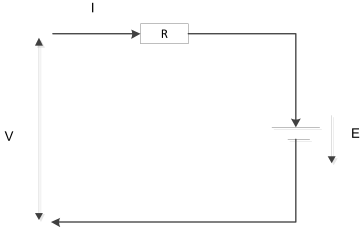
\includegraphics[width=0.9\textwidth, height=0.9\textheight, keepaspectratio=true]{media/image7528.svg.png}
\caption{Electrical equivalent model for KiBaM \protect \label{fig:electrical-equivalent-model-for-kibam}}
\end{figure}

The battery's open circuit voltage is modeled in the same form for charging and discharging, but with different coefficients. The open circuit voltage in charging (\({E_c}\) ) and in discharging (\({E_d}\) ) can be respectively expressed as:

\begin{equation}
{E_c} = {E_{0,d}} + {A_c}{X_c} + \frac{{{C_c}{X_c}}}{{{D_c} - {X_c}}}
\end{equation}

\begin{equation}
{E_d} = {E_{0,c}} + {A_d}{X_d} + \frac{{{C_d}{X_d}}}{{{D_d} - {X_d}}}
\end{equation}

where,

\({E_{0,c}}\) ~~~~~~~~~~~~~~ : Open circuit voltage for a fully charged battery

\({E_{0,d}}\) ~~~~~~~~~~~~~~ : Open circuit voltage for a fully discharged battery

\({A_c}\) , \({C_c}\) , \({D_c}\) ~~~: Constant parameters for charging

\({A_d}\) , \({C_d}\) , \({D_d}\) ~~: Constant parameters for discharging

\({X_c}\) , \({X_d}\) ~~~~~~~~: Normalized maximum capacity at a given charging or discharging current, calculated as:

\begin{equation}
X = \left\{
    \begin{array}{cl}
      q_0 / q_{max}(I) & \; (charging) \\
      (q_{max}-q_0)/q_{max}(I) & \; (discharging)
    \end{array}
  \right.
\end{equation}

It needs to be noted that the performance curve (Curve:RectangularHyperbola2) used in the model input covers the 2\(^{d}\) and the 3\(^{d}\) item of the open circuit voltage equation. Due to the reformatting of performance curve, the voltage function regression coefficients can map to the curve coefficients as follows:

\({C_1} = - C\) ~;\({C_2} = - D\) ;\({C_3} = A\)

With open circuit voltage, the battery terminal voltage (V) can be calculated as:

\begin{equation}
V = E - IR
\end{equation}

where, R is the battery internal resistance in Ohms; the current is positive for discharging and negative for charging.

Given desired power in/out of the battery, the desired charge or discharge current can be calculated from the basic power equation: \(P = VI\) . In this calculation, iteration is needed to ensure the electric current has converged and the battery operation satisfies all specified technical constraints such as maximum discharge current and charge rate limit.

KiBaM assumes that battery life is a primary function of charge/discharge cycles. One cycle is defined as the process of starting from a certain state of charge (SOC), the battery is discharged to a lower SOC and then recharged back to the starting SOC. It is regarded that the magnitude of cycle plays more important than the average of SOC during the cycle. This means that in terms of the impact on battery life, the cycle from 90\% to 70\% and then recharge back to 90\% of SOC is equivalent to another cycle from 50\% to 30\% and then recharge back to 50\% of SOC.~ Battery life in terms of the number of cycles is predicted as a function of the cycle range measured by the fractional depth of discharge. A double exponential equation is used to capture the damage to batteries due to cycling. The equation takes the following form where the coefficients need to be derived from battery test data via curve fitting.

\begin{equation}
{C_F} = {C_1} + {C_2}{e^{{C_3}R}} + {C_4}{e^{{C_5}R}}
\end{equation}

where,

\({C_F}\) ~~~ :~~~ Cycles to failure

\({C_1}\) -\({C_5}\) :~~~ Regression coefficients

R~~~~~~ :~~~ Cycle range in terms of fractional SOC

Following Hybrid2, the rainflow counting method (Downing and Socie 1982) is used to count battery cycles within a state of charge time series. Based on the number of cycles for each fractional SOC range, the battery damage is estimated as:

\begin{equation}
D = \sum\limits_{i = 1}^{} {\left( {{N_i}\frac{1}{{{C_{F,i}}}}} \right)}
\end{equation}

where,

D~~~ : Fractional battery damage. For example, a value of 0.5 at the end of simulation means that half of the battery life is used up after the length of the simulation period.

\({C_{F,i}}\) : Number of cycles to failure for the i-th cycle range

\({N_i}\) ~ : Total number of cycles over the simulation with the i-th cycle range

It needs to be noted that the temperature effects on battery performance and battery self-discharge are not supported in the current model.

\subsubsection{References}\label{references-021}

Bindner H., Cronin T., Lundsager P., Manwell J.F., Abdulwahid U., and Baring-Gould I. 2005. Lifetime Modeling of Lead Acid Batteries. Riso National Laboratory, Roskilde, Denmark.

Downing S. D. and Socie D. F. 1982.~ Simple rainflow counting algorithms, International Journal of Fatigue, 1982.

Manwell J. F. and McGowan J. G. 1993. A lead acid battery storage model for hybrid energy systems, Solar Energy 50(5): 399- 405.

\subsection{Electric Load Center Transformers}\label{electric-load-center-transformers}

Transformers (object name: ElectricLoadCenter:Transformer) are an integral part of the electric distribution system. They have two broad applications closely related to building energy simulation. First, transformers are used to lower the voltage of electricity from utility primary circuits to customer secondary circuits, and in this case they are called distribution transformers. Second, transformers are used to output the surplus power from onsite generators to the electricity grid.

Distribution transformers reduce the voltage on utility distribution lines (34.5 kV or less) to a lower secondary voltage (600 V or less) suitable for customer equipment. Distribution transformers are usually categorized according to the medium used for cooling and insulation (liquid or air), the voltage class that they serve (low or medium), and the number of phases (single phase or three phase).

Liquid-immersed transformers rely on oil or other fire resistant liquid around the coils for cooling. In contrast, dry type transformers rely only on the natural convection of air for insulation and cooling. Medium-voltage transformers step from utility line voltage down to a lower secondary voltage, depending on the application. The secondary voltage from a medium-voltage transformer is usually at 277 V for single phase and 480 V for three phase. This secondary voltage can be directly used as 480 V three-phase power for large motors or as 277 V single-phase power for some fluorescent lighting. However, for most industrial and commercial facilities, low-voltage transformers are needed to reduce the above voltages further to 208/120 V. Common 120 V loads are wall plugs and incandescent lighting.

Most liquid-immersed transformers are owned by utilities and they are of the medium-voltage type. Virtually all dry type transformers are owned by commercial and industrial customers (Barnes et al. 1996). Of the dry type transformers, those of the medium-voltage type are generally special-order items while those of the low-voltage type are commodity items. The efficiency requirement of distribution transformers is covered by the NEMA (National Electrical Manufactures Association) Standard TP 1. ASHRAE 90.1-2010 will cite the NEMA Standard TP 1 to stipulate the efficiency requirement for the low-voltage dry type distribution transformers.

There are two main types of energy losses in transformers: no load loss and load loss. The no load loss comes primarily from the switching of the magnetic fields in the core material. Hence, it is also called the core loss. The no load (core) loss is roughly constant and exists continuously in the core material as long as the transformer is energized. The load loss comes from the electrical resistance in the windings when there is a load on the transformer. Hence, the load loss is also called the winding loss. The load (winding) loss is proportional to the load squared with a small temperature correction.

Given the no load loss (NL) and the load loss (LL) at rated load and conditions, the total energy losses in a transformer at time t is calculated as:

\begin{equation}
TL(t) = NL + LL(t) = NL + LL*P{(t)^2}*{f_T}(t)
\end{equation}

where,

\(TL(t)\) ~~~~~~~ Total energy loss at time t (W)

\(LL(t)\) ~~~~~~~ Load loss at time t (W)

\(P(t)\) ~~~~~~~~~ Per unit load at time t

\({f_T}(t)\) ~~~~~~~~ Temperature correction factor for the load loss at time t

The per unit load at time t is calculated as:

\begin{equation}
P(t) = \frac{{Load(t)}}{{{S_B}}}
\end{equation}

where,

\(Load(t)\) Transformer load at time t (W)

\({S_B}\) Transformer nameplate rating (VA)

The temperature correction factor at time t is calculated as (NEMA 2002):

\begin{equation}
{f_T}(t) = {L_{dc}}*\frac{{R(t)}}{{{R_{ref}}}} + {L_{eddy}}*\frac{{{R_{ref}}}}{{R(t)}}
\end{equation}

where,

\({L_{dc}}\) ~~~~~~~~~~~ Per unit load loss due to electrical resistance

\({L_{eddy}}\) ~~~~~~~~~ Per unit load loss due to eddy currents

\(R(t)\) ~~~~~~~~~ Winding electrical resistance at time t

\({R_{ref}}\) ~~~~~~~~~~ Winding electrical resistance at the full load reference conditions

The ratio of winding electrical resistance is calculated as:

\begin{equation}
\frac{{R(t)}}{{{R_{ref}}}} = \frac{{F + {T_{winding}}(t) + {T_{amb}}(t)}}{{F + {T_{winding,ref}} + {T_{amb,ref}}}}
\end{equation}

where,

\(F\) ~ Thermal coefficient of resistance for the winding material ( = 225 for aluminum and 234.5 for copper)

\({T_{winding,ref}}\) Winding temperature rise at the full load reference conditions (°C)

\({T_{winding}}(t)\) Winding temperature rise at time t (°C)

\({T_{amb,ref}}\) ~~~~~~ Ambient temperature at the reference condition ( = 20 °C)

\({T_{amb}}(t)\) ~~~~~ Ambient temperature at time t (°C)

The Ambient temperature \({T_{amb}}(t)\) is equal to the zone temperature if a thermal zone is specified in the input; otherwise, it is assumed equal to 20 °C. The winding temperature rise at time t is calculated as (Barnes et al. 1997):

\begin{equation}
{T_{winding}}(t) = P{(t)^{1.6}}*{T_{winding.ref}}
\end{equation}

Based on the derived total energy losses in a transformer, the transformer efficiency at time t can be calculated according to the following equation:

\begin{equation}
\eta (t) = \frac{{Load(t)}}{{Load(t) + NL + LL(t)}}
\end{equation}

The above procedure describes how to calculate the total transformer energy losses based on the no load loss and load loss at rated conditions. The transformer model also supports the case when the nominal transformer efficiency is given. In this case, the user needs to provide the nameplate efficiency and the corresponding per unit load, the maximum efficiency and the corresponding per unit load, and the reference conductor temperature at which the nameplate efficiency is measured. Given these information, both no load loss and load loss at rated conditions can be derived as below.

The nameplate efficiency can be expressed as:

\begin{equation}
{\eta_{np}} = \frac{{{S_B}*{P_{np}}}}{{{S_B}*{P_{np}} + NL + LL*P_{np}^2*{f_{T,np}}}}
\end{equation}

where,

\({\eta_{np}}\) ~~~~~~~~~~~ Nameplate efficiency

\({S_B}\) Nameplate rating (VA)

\({P_{np}}\) ~~~~~~~~~~~ Per unit load at which the nameplate efficiency is measured

\({f_{T,np}}\) ~~~~~~~~~ Applied temperature correction factor for the nameplate efficiency

Maximum efficiency generally occurs when the load loss is equal to the no-load loss. Because the no-load loss does not vary with the load on the transformer, the following relationship can be established:

\begin{equation}
NL = L{L_{\max ,\eta }} = LL*P_{\max ,\eta }^2*{f_{T,\max  - \eta }}
\end{equation}

where,

\({P_{\max ,\eta }}\) ~~~~~~~~ Per unit load at which the maximum efficiency is obtained

\({f_{T,\max - \eta }}\) ~~~~ Applied temperature correction factor for the maximum efficiency

Transformers typically have close per unit loads for the nameplate efficiency and the maximum efficiency. Therefore, it is reasonable to assume that the applied temperature correction factors are equal at those two efficiencies. This implies that:

\begin{equation}
\frac{{L{L_{np}}}}{{L{L_{\max ,\eta }}}} = \frac{{LL*{P_{np}}^2*{f_{T,np}}}}{{LL*{P_{\max ,\eta }}^2*{f_{T,\max  - \eta }}}} = {\left( {\frac{{{P_{np}}}}{{{P_{\max ,\eta }}}}} \right)^2}
\end{equation}

Rearranging Equation and combining it with Equation leads to:

\begin{equation}
L{L_{np}} = L{L_{\max ,\eta }}*{\left( {\frac{{{P_{np}}}}{{{P_{\max ,\eta }}}}} \right)^2} = NL*{\left( {\frac{{{P_{np}}}}{{{P_{\max ,\eta }}}}} \right)^2}
\end{equation}

Combining Equations and , we can obtain the no load loss as:

\begin{equation}
NL = \frac{{{S_B}*{P_{np}}*(1 - {\eta_{np}})}}{{{\eta_{np}}*\left[ {1 + {{\left( {\frac{{{P_{ref}}}}{{P{}_{\max ,\eta }}}} \right)}^2}} \right]}}
\end{equation}

Substitute NL into Equation , we can calculate the load loss at rated conditions as:

\begin{equation}
LL = \frac{{NL}}{{{f_{T,\max  - \eta }}*P_{\max ,\eta }^2}} = \frac{{NL}}{{{f_{T,np}}*P_{\max ,\eta }^2}}
\end{equation}

Since both no load and load losses at rated conditions are known, the total energy losses in a transformer at time t can then be calculated according to Equation

\subsubsection{References:}\label{references-1-008}

Barnes, PR., JW. Van Dyke, BW. McConnell, and S. Das. 1996. Determination Analysis of Energy Conservation Standards for Distribution Transformer, ORNL-6847. Oak Ridge National Laboratory, Oak Ridge, TN.

Barnes, PR., S. Das, BW. McConnell, and JW. Van Dyke. 1997. Supplement to the ``Determination Analysis'' (ORNL-6847) and Analysis of the NEMA Efficiency Standard for Distribution Transformer, ORNL-6925. Oak Ridge National Laboratory, Oak Ridge, TN.

NEMA. 2002. NEMA Standards Publication TP 1-2002: Guide for Determining Energy Efficiency for Distribution Transformers. National Electrical Manufactures Association, Rosslyn, VA.
